\section{Results}

This section analyzes the collective behaviors of motorcycle taxi drivers using helmet-mounted sensor data (air quality, location, movement) to understand how individual PM2.5 exposure varies across time periods and locations, and how drivers subsequently respond based on these observed exposure patterns.

\begin{figure*}
    \centering
    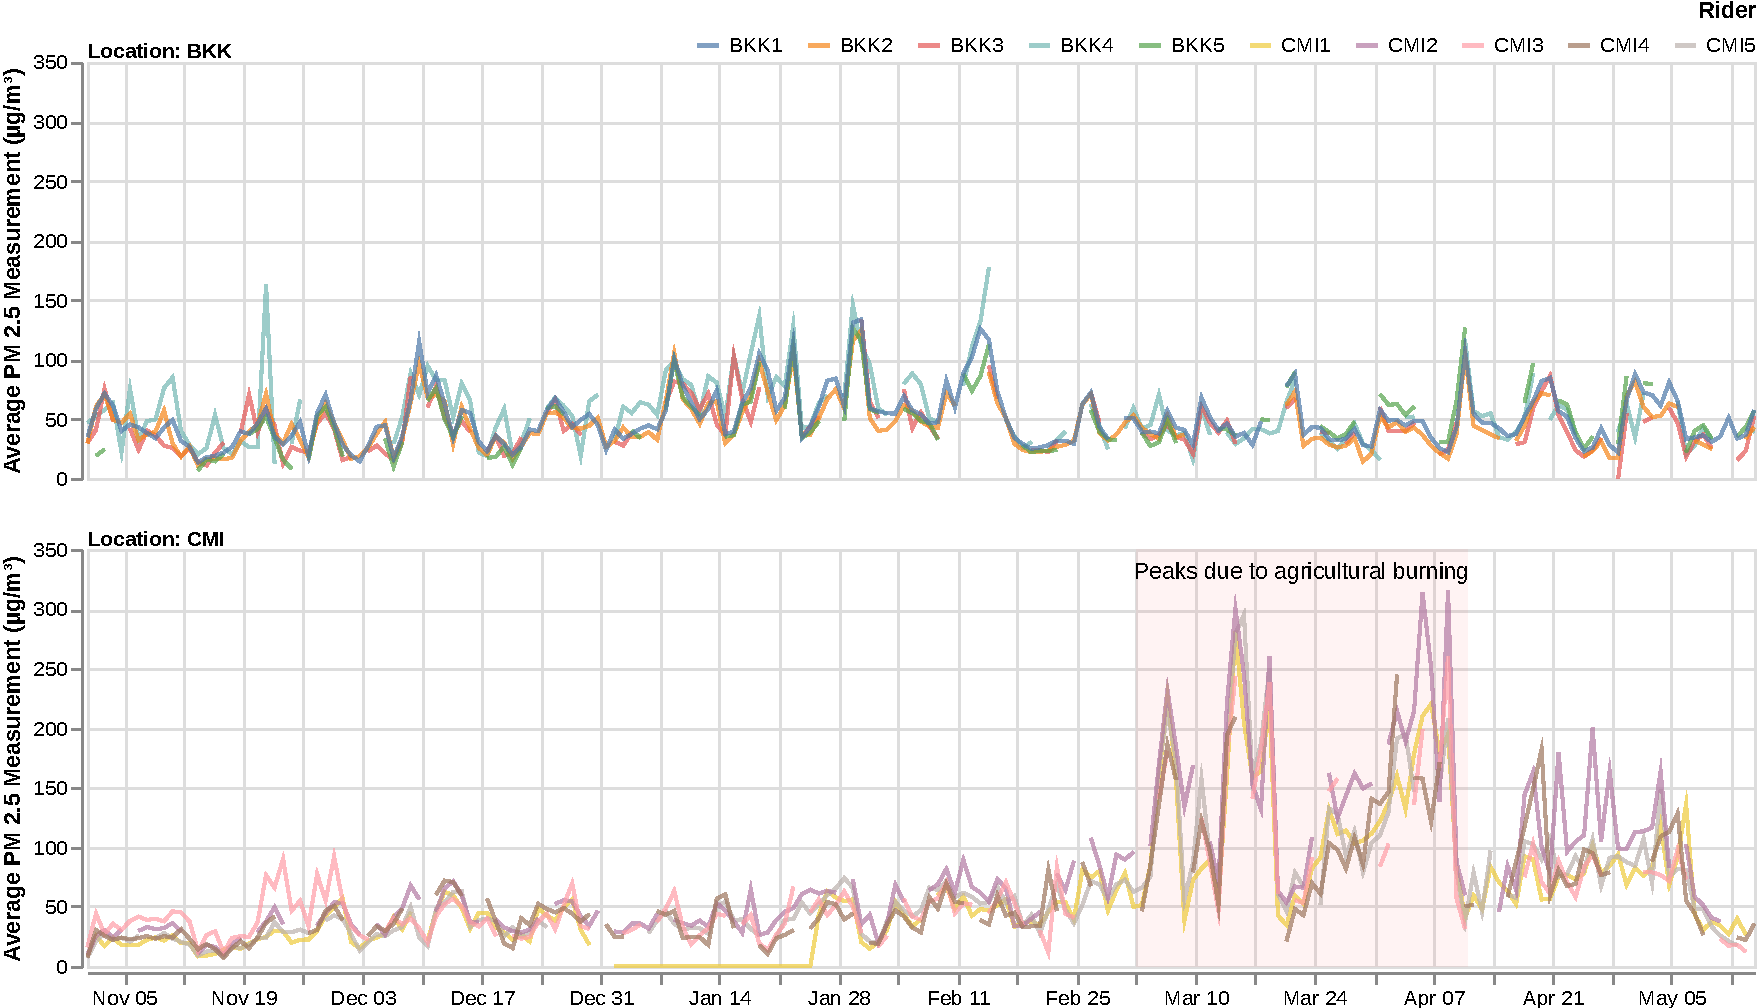
\includegraphics[width=\textwidth]{figures/daily-pollution-per-rider.pdf}
    \caption{
    Daily PM 2.5 exposure measured from the helmet-mounted sensors for Bangkok and Chiang Mai drivers.
    Vertical grid lines represent Sundays.
    }
    \Description{}
    \label{fig:daily-pollution-per-driver}
\end{figure*}

\subsection{PM2.5's Temporal Patterns}
Analyzing daily average PM2.5 exposure (\autoref{fig:daily-pollution-per-driver}) reveals relatively consistent levels in Bangkok (BKK), peaking moderately from December to mid-February,
while Chiang Mai (CMI) shows pronounced seasonality with extreme peaks from March to early April (consistent with agricultural burning periods~\cite{david2025chiangmaiburn, bernsten2024chiangmaiburn, iqair2023chiangmaiburn}).
Within each city, drivers experience similar daily trends.
Hourly averages (\autoref{fig:hourly-work-aqi}) show daily cycles peaking during morning (BKK: 7 AM, CMI: 8 AM) and evening rush hours, with an afternoon dip, although late night/early morning data shows higher variance.
Notably, BKK's PM2.5 measurements show a consistent trend throughout the year, reinforcing traffic as the primary air pollution source.
In contrast, CMI's dominant seasonal variation indicates agricultural burning as the primary driver.
Thus, PM2.5 sources differ substantially between cities (BKK: traffic, CMI: agricultural burning), implying the need for location-specific mitigation strategies.



\begin{figure*}
    \centering
    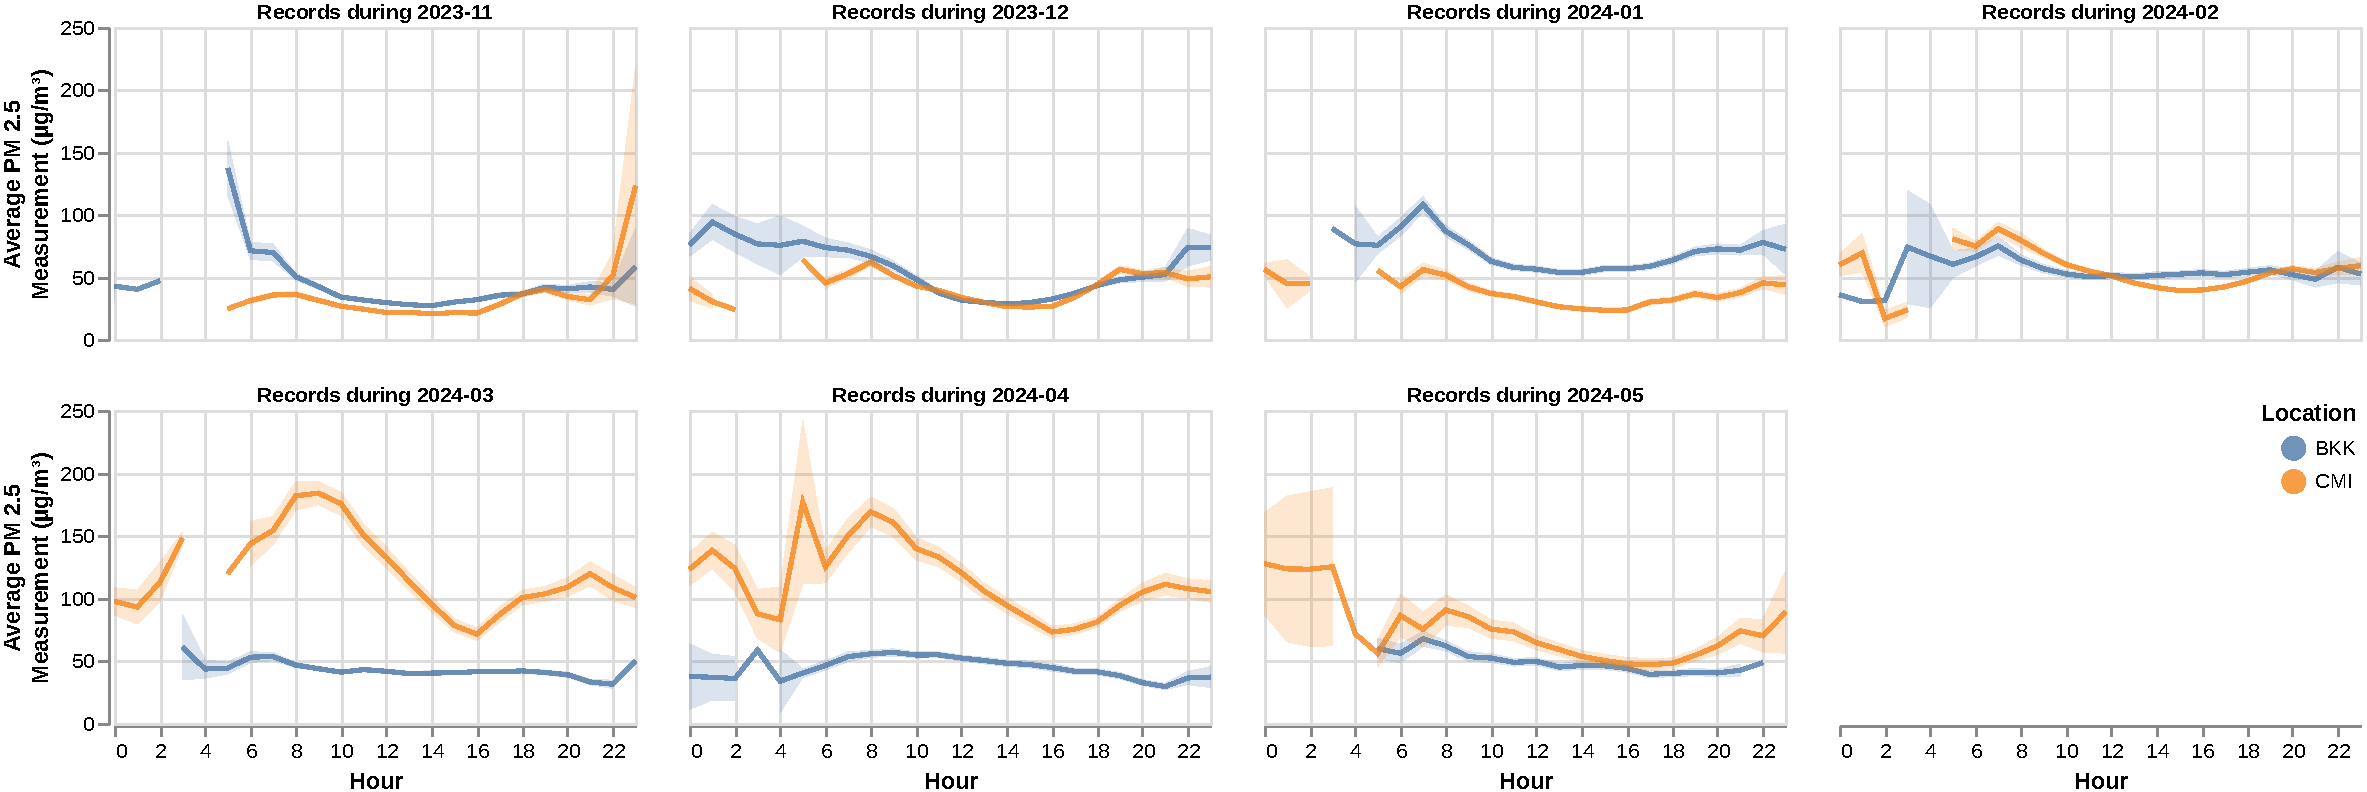
\includegraphics[width=\textwidth]{figures/average-hourly-pollution.pdf}%
    \caption{Mean and standard deviations of air pollution measurement in each hour of the day throughout the study period.
    Each subplot represents each month in the study. }%
    \Description{}
    \label{fig:hourly-work-aqi}%
\end{figure*}%



\subsection{PM2.5's Spatial Patterns}

Spatial analysis (\autoref{fig:subdistrict-aqi}) reveals that PM2.5 distribution is uneven across subdistricts and individual drivers, with drivers experiencing different exposure levels even in similar areas.
Furthermore, each driver tends to operate primarily within specific locations.
Consequently, effective PM2.5 exposure mitigation strategies must consider these individual spatial work patterns.



\begin{figure*}[t]
    \centering

    \begin{subfigure}[t]{0.49\textwidth}
        \centering
        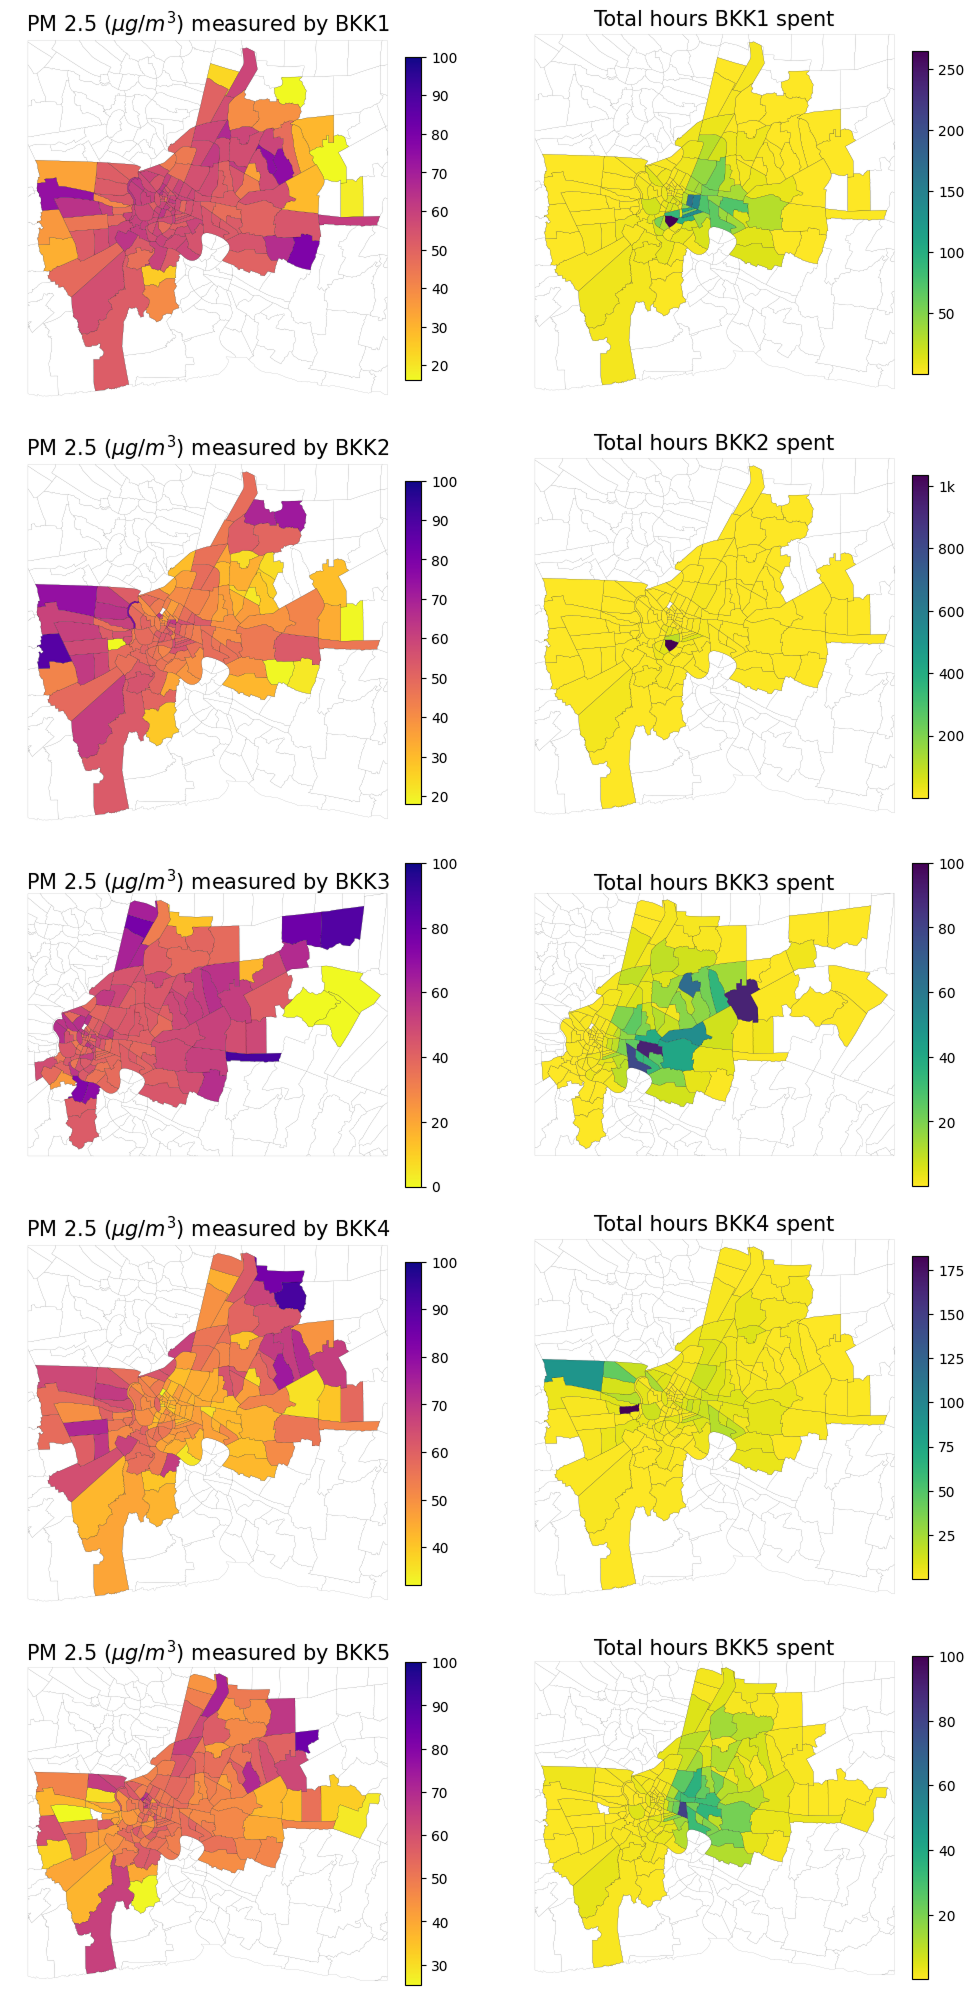
\includegraphics[width=\linewidth]{figures/map/BKK_PM_TIME.png}%
        \caption{Measurement collected in Bangkok.}
    \end{subfigure}%
    \hfill
    \begin{subfigure}[t]{0.49\textwidth}
        \centering
        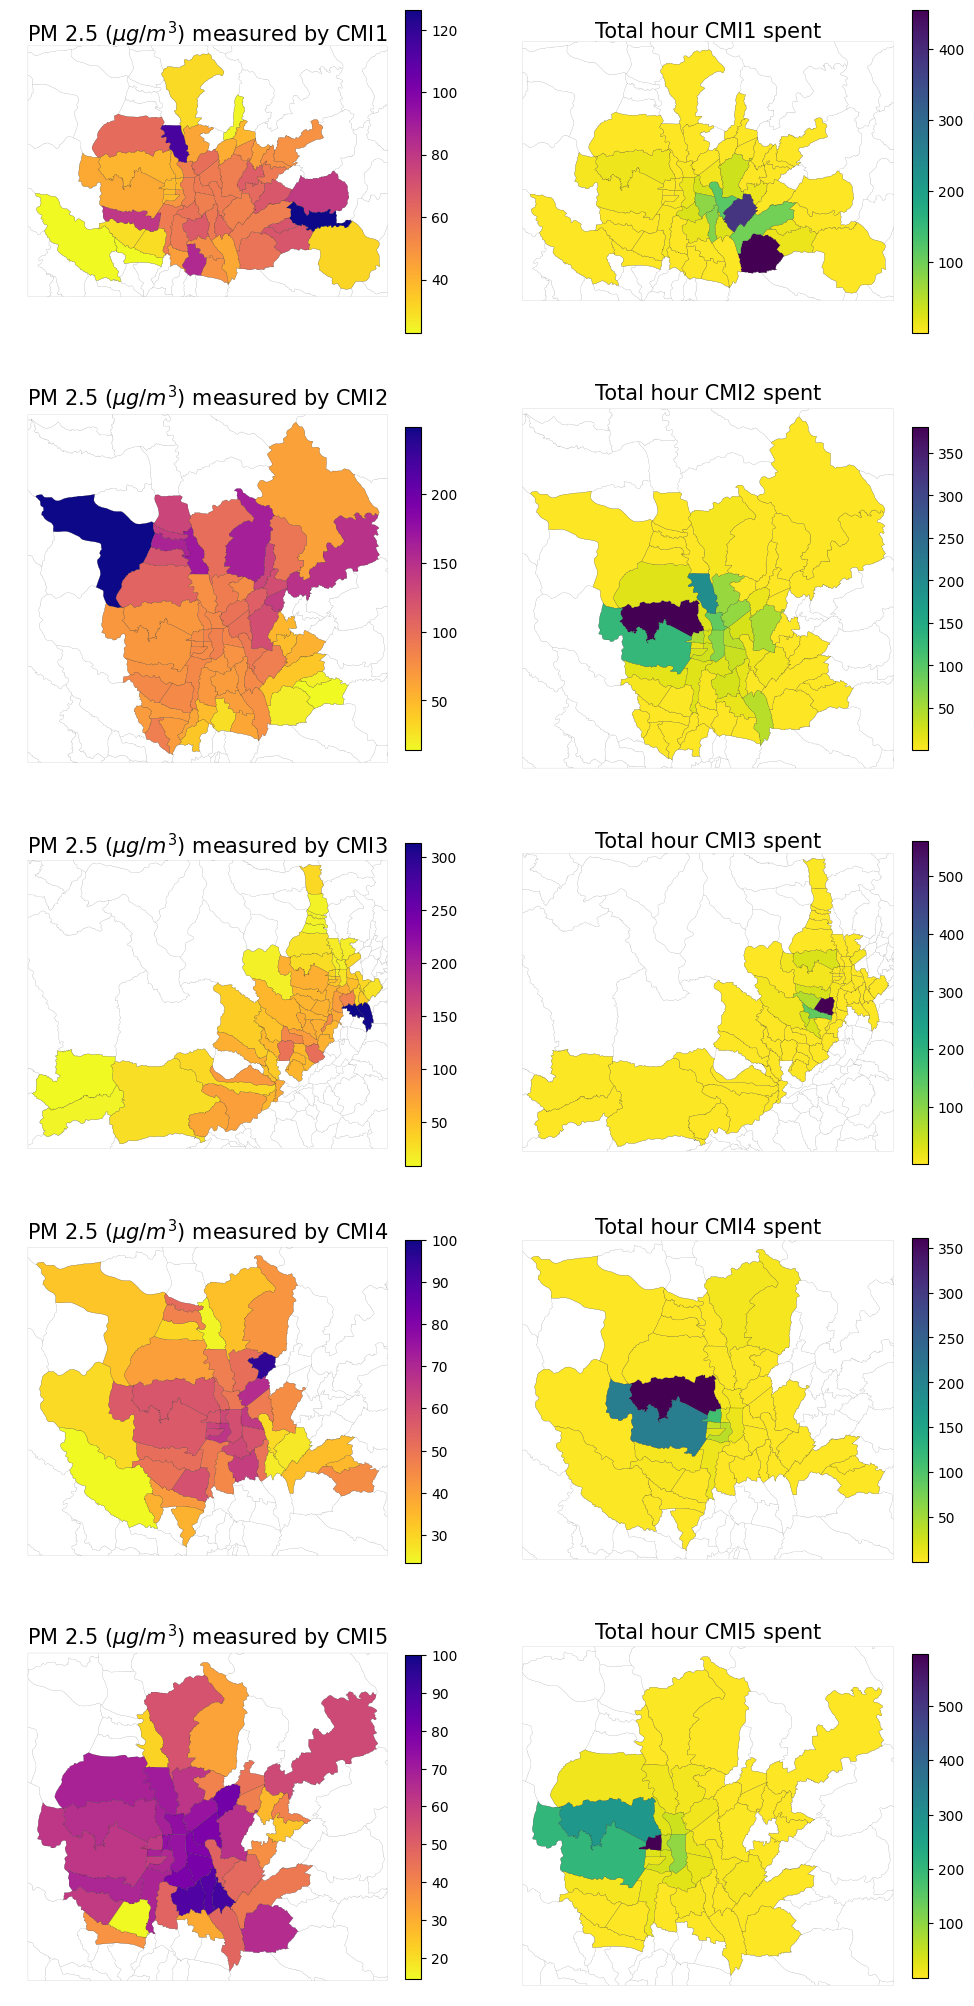
\includegraphics[width=\linewidth]{figures/map/CMI_PM_TIME.png}%
        \caption{Measurement collected in Chiang Mai.}
    \end{subfigure}%

    \caption{
    The left column of each sub-figure shows the average PM2.5 level throughout the study period measured in each subdistrict.
    The right column of each sub-figure shows the amount of time in hours that each driver spent in each subdistrict throughout the study.
    }
    \Description{}
    \label{fig:subdistrict-aqi}
\end{figure*}


 
